% TODO https://fidoalliance.org/specifications/
% TODO https://fidoalliance.org/overview/history/

\section{History and evolution}

The \wa{} is an outcome of joint efforts from the \gls{fido} alliance and and the \gls{w3c}. It is a product from various preceding industry standards, namely \gls{uaf} and \gls{u2f}. This chapter introduces the origin of the \wa{} by explaining the origin of the \gls{fido} alliance and their works on the \gls{uaf} and \gls{u2f} with a focus of the technical implementations, protocols and used techniques.

\subsection{FIDO Alliance}

The \gls{fido} alliance is an open industry association founded in July 2012 and launched in February 2013. Companies such as PayPal, Lenovo, and Infineon founded the \gls{fido} alliance. Currently the alliance has more than 260 members, including, e.g., Google, Amazon, Yubico, Samsung, Microsoft, VISA, or MasterCard. The goal of the \gls{fido} alliance is to develop new authentication protocols and standards in order to enhance and simplify the user experience of \gls{mfa} and to reduce the over usage of passwords.\footcites[See][583]{eckert-it-sec-9}

The \gls{fido} alliance developed the specifications \gls{uaf} and \gls{u2f}. The first specification of the \gls{u2f} was the starting point for the development of the \wa{} in a joint efforts with the \gls{w3c}. The \gls{ctap} is based on the \gls{u2f} specification 1.2 which complements the \wa. Both projects are part of the FIDO2 project.\footcite[See][169--170]{grimes2017hacking}

\subsection{Universal Authentication Framework}

The \glsfirst{uaf} is \gls{fido}'s solution for a passwordless experience. It uses local and native device authentication such as biometrics to authorize the user. It does not feature \gls{2fa}, but is instead meant as direct replacement for the login with passwords. It is based on public key cryptography with the use of challenge-response authentication. The goal of the \gls{uaf} is to provide a generic \gls{api} which enables interoperability and unified user experience. between the different operating systems and clients.

It features three key components, the \gls{uaf} client, the \gls{uaf} server and the \gls{uaf} authenticators. Besides that, the alliance offers a metadata service. The communication between the client and the authenticator is done via the \gls{uaf} \gls{asm}, which offers a standardized solution for the client to access and detect the various different authenticators.

\begin{figure}[hbt]
	\centering
	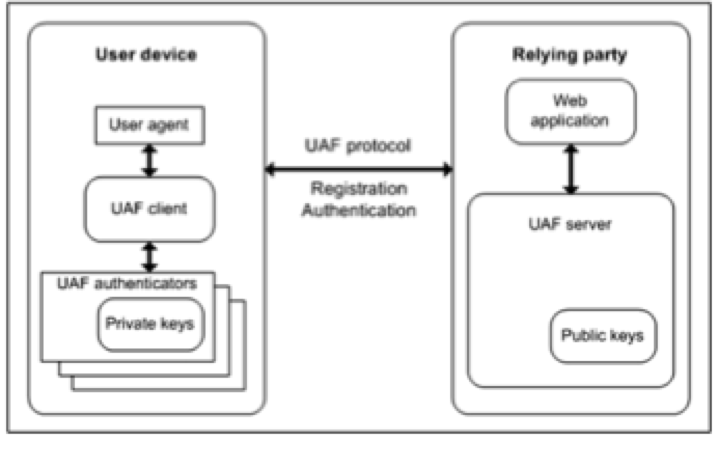
\includegraphics[width=\textwidth]{pics/Picture1}
	\caption[\gls{uaf} architecture overview]{\gls{uaf} architecture overview\footnotemark}
	\label{fig:uaf_architecture}
\end{figure}
\footcitetext[Source: diagram by author, based on][4]{uaf-overview}

\autoref{fig:uaf_architecture} shows the \gls{uaf} architecture, where the client is responsible for the communication between the authenticator, the \gls{fido} client and the corresponding web browser or (mobile) app.

\footcites[See][191]{7897543}[See][131]{10.1007/978-3-319-67639-5_11}[See][]{uaf-asm}


\subsection{Universal Second Factor}

The \glsfirst{u2f} is the second standard developed by the \gls{fido} alliance before the \wa. It explicitly defines the use of a second factor for the password-based login flow which is backed by public-key cryptography. It's contributed by Google and Yubico, both being alliance members. The \textit{strong second factor} can be either connected or disconnected, e.g, built in hardware or for instance an \gls{usb} token, \gls{nfc}-capable device or a standalone \gls{ble} dongle. The protocol defines two layers:

\begin{enumerate}
	\item the first defines the cryptographic basics of the protocol
	\item the second layer defines the communication between the user's authenticator and the first layer over the chosen transport protocol (e.g., \gls{usb}, \gls{nfc}, or \gls{ble}
\end{enumerate}

Besides that, the \gls{u2f} protocol only specifies \gls{usb}, both internal and external \gls{hid} devices, \gls{nfc} and Bluetooth, as well as the low energy variant, \gls{ble}, as possible transport protocols.

\footcites[See][1--2, 4]{u2f-overview}[See][4]{u2f-js-api}

Further, \gls{u2f} has also been renamed to \gls{ctap}1 since the release of the \wa{} to avoid confusion and better understanding that it is usable with the \wa{} as a \gls{ctap}.

\subsection{FIDO2}

\begin{figure}[hbt]
	\centering
	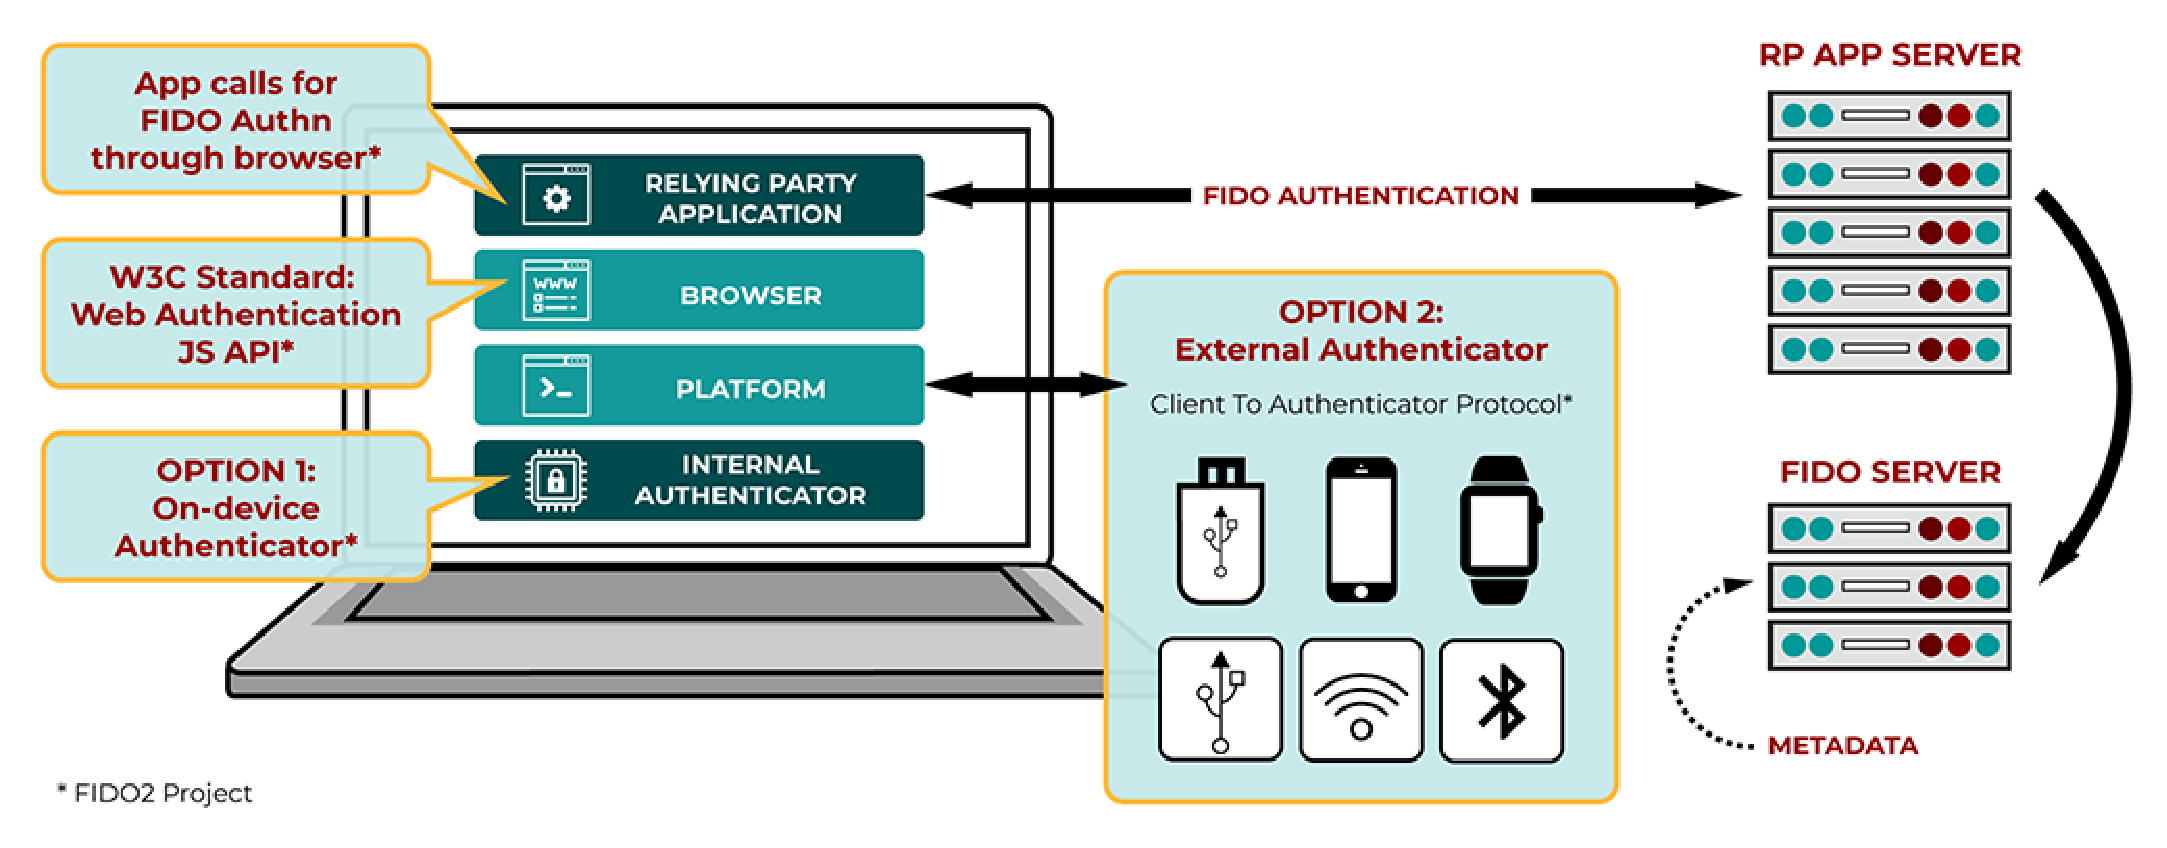
\includegraphics[width=\textwidth]{pics/FIDO2-Graphic-v2}
	\caption[\gls{fido}2 architecture overview]{\gls{fido}2 architecture overview\footnotemark}
	\label{fig:fido2_architecture}
\end{figure}
\footcitetext[Source: https://fidoalliance.org/specifications/][4]{uaf-overview}


\subsubsection{Client to Authenticator Protocol 2}

\subsubsection{Web Authentication API}

The \wa{} is backwards compatible to the \gls{u2f} compatible, thus making every security token that is usable for \gls{u2f} compatible with the \wa, too.